\documentclass[letterpaper]{article} 

% \documentclass[]{article}



\usepackage{geometry}
\geometry{letterpaper, top=3.5cm, left=2cm, right=3.5cm, bottom=1.0cm}

\usepackage[compact]{titlesec}
\usepackage[document]{ragged2e}
\usepackage{multirow}
\usepackage{colortbl}

    \usepackage{lmodern}
    \usepackage{amssymb,amsmath}
\usepackage{ifxetex,ifluatex}
\usepackage{fixltx2e} % provides \textsubscript
\ifnum 0\ifxetex 1\fi\ifluatex 1\fi=0 % if pdftex
\usepackage[T1]{fontenc}
\usepackage[utf8]{inputenc}

\usepackage{color}


% pandoc syntax highlighting
  
    
% graphix
\usepackage{graphicx}
\setkeys{Gin}{width=\linewidth,totalheight=\textheight,keepaspectratio}

% booktabs
\usepackage{booktabs}

% float images
\usepackage{wrapfig}

\usepackage{array}


\usepackage[scaled]{helvet}
\renewcommand\familydefault{\sfdefault} 
\usepackage[T1]{fontenc}


\renewcommand{\arraystretch}{0}
\usepackage{ejbi}

\usepackage{fancyhdr}

\pagestyle{fancy}
\fancyhf{}
\fancyhead[LE,RO]{
\includegraphics[width=50mm]{logo.png}}

% \pagestyle{fancy}
% \fancyhf{}
% \fancyhead[R]{
\includegraphics[width=50mm]{logo.png}}
% \fancyfoot[R]{hola}
% % 
% % \setlength{\headheight}{10.50mm}
% \pagestyle{fancy}

\begin{document}



\begin{table}[h!]
 \setlength{\tabcolsep}{0pt}
\def\arraystretch{0}
  \begin{tabular}{m{4cm}m{12cm}}

    &
    \vspace{10pt} 

                \begin{center}
        \begin{ejbi-title}
        Del contrato yo me encargo
        \end{ejbi-title}
        \end{center}
        %\bigskip
                      \begin{center}
      \begin{ejbi-subtitle}
      Cargos a Alcalde de Solano (2012-2015) por irregularidades en contratos
      de salud
      \end{ejbi-subtitle}
      \end{center}
      %}
      %\bigskip
        \end{tabular}
%  \egroup
\end{table}


%\begin{abstract}
\color{colT}{\justify{En 2014, Yecson Peña Ceballos, entonces secretario de Gobierno del
municipio de Solano (Caquetá), junto con el entonces alcalde Eliseo
Murillo Criollo (2012-2015) firmaron un contrato con la IPS privada
Grupo Empresarial Viamad Ltda sin contar con las respectiva autorización
por parte de la Secretaría de Salud del Caquetá. Además el secretario de
Gobierno era el alcalde encargado en el momento de abrir la convocatoria
para seleccionar a los contratistas. En enero de 2018 se le imputaron
cargos al alcalde y al secretario por desconocer los principios de
economía, responsabilidad y transparencia en la contratación pública,
siendo esta una falta calificada como gravísima.}}
%\end{abstract}


\vspace{0.5cm}

\begin{center}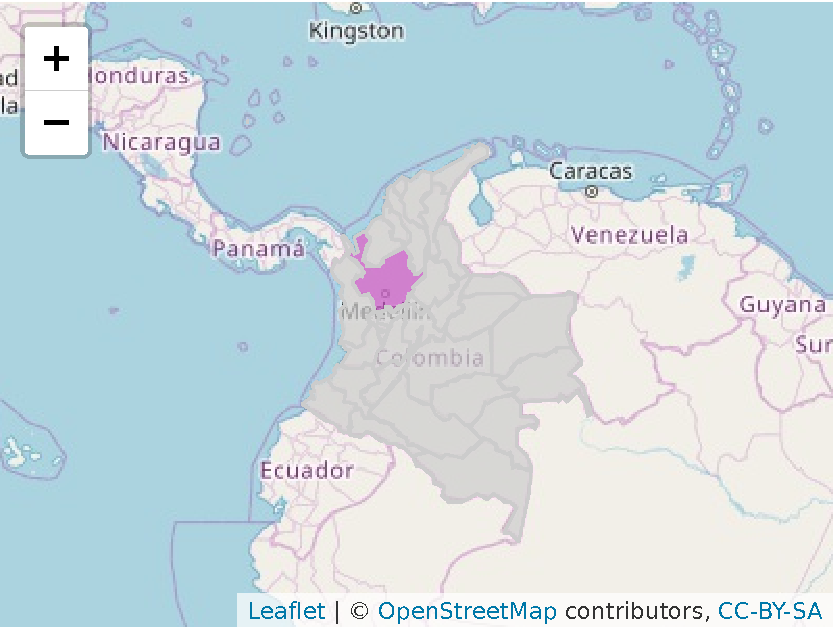
\includegraphics[width=150px,height=150px]{built_report_files/figure-latex/unnamed-chunk-2-1} \end{center}
  

  
\vspace{0.5cm}

\begin{minipage}[t]{0.45\textwidth}%
  
\begin{tabular}{m{3.4cm}m{3.6cm}}
 \begin{ejbi-colone}LUGAR DEL HECHO:\end{ejbi-colone}& 
  \begin{ejbi-coltwo} CAQUETA \end{ejbi-coltwo}\\ 
 \colrul 
 \addlinespace
 \begin{ejbi-colone}FECHA DEL HECHO:\end{ejbi-colone} &
  \begin{ejbi-coltwo} 2014 \end{ejbi-coltwo}   \\
 \colrul 
 \addlinespace
 \specialcell[]{\begin{ejbi-colone}ACTOR O ENTIDAD\end{ejbi-colone} \\
 \addlinespace
 \begin{ejbi-colone}INVOLUCRADO: \end{ejbi-colone}}&
  \begin{ejbi-coltwo} (Alcalde (2012015)). (Secretario de Gobierno (2012015)) \end{ejbi-coltwo} \\ 
\addlinespace\colrul
 \addlinespace
 \specialcell[]{\begin{ejbi-colone}TIPO DE \end{ejbi-colone}\\ 
 \begin{ejbi-colone}CORRUPCIÓN:\end{ejbi-colone}}&
  \begin{ejbi-coltwo} Corrupción Administrativa \end{ejbi-coltwo} \\
 \addlinespace \colrul
 \end{tabular}
\end{minipage}%
\qquad{\color{colfich}\vrule}\qquad
\begin{tabular}{@{}l@{}}

\begin{tabular}{m{3.6cm}m{3.6cm}}
\begin{ejbi-colone}DERECHO VULNERADO\end{ejbi-colone} &
 \begin{ejbi-coltwo}Derechos sociales, económicos y culturales\end{ejbi-coltwo}\\ 
\colrul
\addlinespace
\begin{ejbi-colone}SECTOR AFECTADO\end{ejbi-colone} &
 \begin{ejbi-colone}SALUD\end{ejbi-colone}\\ 
\colrul
\addlinespace
\multicolumn{1}{c !{\color{colfich}\vline}}{{\begin{tabular}{@{}c@{}}
 \\
 \\
 \begin{ejbi-colone}ENTIDAD DE\end{ejbi-colone}\\\addlinespace \begin{ejbi-colone}CONOCIMIENTO:\end{ejbi-colone}\end{tabular} }} & 
 \multicolumn{1}{c}{\begin{ejbi-colone}ESTADO JUDICIAL:\end{ejbi-colone}} 
 \\
 \multicolumn{1}{c !{\color{colfich}\vline}}{{\begin{ejbi-coltwo} \parbox[t]{3.4cm}{\begin{center}Alcaldía Municipal de Solano-Caquetá\end{center}}\end{ejbi-coltwo}}}  & \multicolumn{1}{c}{\begin{ejbi-coltwo}\parbox[t]{3.4cm}{\begin{center} Imputado\end{center}} \end{ejbi-coltwo}} \\ \arrayrulecolor{colfich}\hline
\end{tabular}
\end{tabular}

\vspace{1cm}

\begin{flushright}
\textit{Última actualización 2018-01-11 05:00:00} 
\end{flushright}

\end{document}